%!TEX root = ../main.tex
\begin{frame}{Différents stades de l'expansion d'un porte-feuille}
  \textit{Il était une fois ...}
  \begin{figure}[tb]
    \centering
    \includegraphics<1>[width=0.99\textwidth]{figures/schema_optimisation0.pdf}
    \includegraphics<2>[width=0.99\textwidth]{figures/schema_optimisation1.pdf}
    \includegraphics<3>[width=0.99\textwidth]{figures/schema_optimisation2.pdf}
    \includegraphics<4>[width=0.99\textwidth]{figures/schema_optimisation3.pdf}
  \end{figure} 
\end{frame}

% \begin{frame}{Optimisation}
% \vspace{-10pt}
% \textit{Fonction objective : } Fonction de qualité d'une solution\\
% \textit{Contrainte : } Conditions à respecter\\ 
% \vspace{0.4cm}
% \hrule
% \vspace{0.3cm}
% \pause
% \textbf{Exemple}
%   \begin{figure}[h!]
%     \centering
%     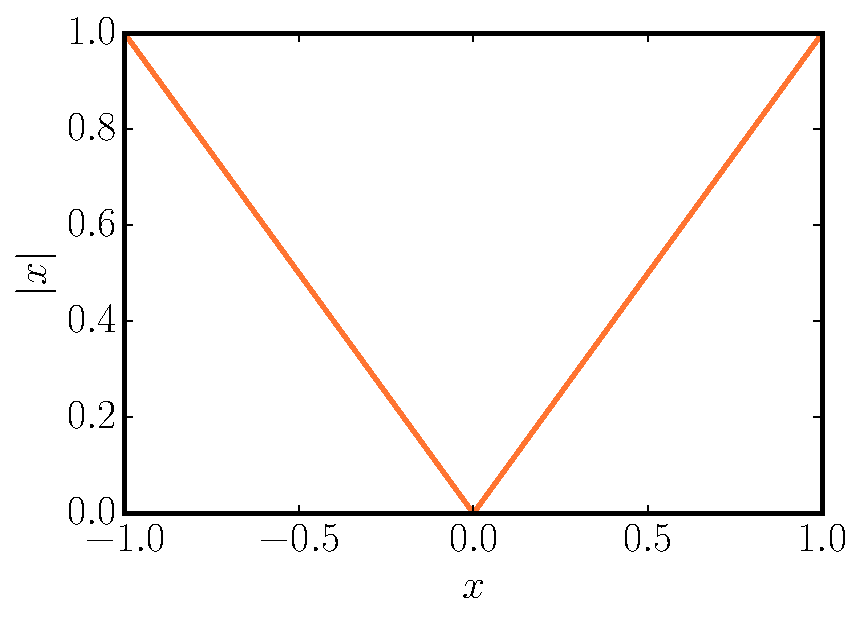
\includegraphics[width=0.60\textwidth]{figures/absolute_function.pdf}
%   \end{figure}
% \end{frame}